\documentclass[1p]{elsarticle_modified}
%\bibliographystyle{elsarticle-num}

%\usepackage[colorlinks]{hyperref}
%\usepackage{abbrmath_seonhwa} %\Abb, \Ascr, \Acal ,\Abf, \Afrak
\usepackage{amsfonts}
\usepackage{amssymb}
\usepackage{amsmath}
\usepackage{amsthm}
\usepackage{scalefnt}
\usepackage{amsbsy}
\usepackage{kotex}
\usepackage{caption}
\usepackage{subfig}
\usepackage{color}
\usepackage{graphicx}
\usepackage{xcolor} %% white, black, red, green, blue, cyan, magenta, yellow
\usepackage{float}
\usepackage{setspace}
\usepackage{hyperref}

\usepackage{tikz}
\usetikzlibrary{arrows}

\usepackage{multirow}
\usepackage{array} % fixed length table
\usepackage{hhline}

%%%%%%%%%%%%%%%%%%%%%
\makeatletter
\renewcommand*\env@matrix[1][\arraystretch]{%
	\edef\arraystretch{#1}%
	\hskip -\arraycolsep
	\let\@ifnextchar\new@ifnextchar
	\array{*\c@MaxMatrixCols c}}
\makeatother %https://tex.stackexchange.com/questions/14071/how-can-i-increase-the-line-spacing-in-a-matrix
%%%%%%%%%%%%%%%

\usepackage[normalem]{ulem}

\newcommand{\msout}[1]{\ifmmode\text{\sout{\ensuremath{#1}}}\else\sout{#1}\fi}
%SOURCE: \msout is \stkout macro in https://tex.stackexchange.com/questions/20609/strikeout-in-math-mode

\newcommand{\cancel}[1]{
	\ifmmode
	{\color{red}\msout{#1}}
	\else
	{\color{red}\sout{#1}}
	\fi
}

\newcommand{\add}[1]{
	{\color{blue}\uwave{#1}}
}

\newcommand{\replace}[2]{
	\ifmmode
	{\color{red}\msout{#1}}{\color{blue}\uwave{#2}}
	\else
	{\color{red}\sout{#1}}{\color{blue}\uwave{#2}}
	\fi
}

\newcommand{\Sol}{\mathcal{S}} %segment
\newcommand{\D}{D} %diagram
\newcommand{\A}{\mathcal{A}} %arc


%%%%%%%%%%%%%%%%%%%%%%%%%%%%%5 test

\def\sl{\operatorname{\textup{SL}}(2,\Cbb)}
\def\psl{\operatorname{\textup{PSL}}(2,\Cbb)}
\def\quan{\mkern 1mu \triangleright \mkern 1mu}

\theoremstyle{definition}
\newtheorem{thm}{Theorem}[section]
\newtheorem{prop}[thm]{Proposition}
\newtheorem{lem}[thm]{Lemma}
\newtheorem{ques}[thm]{Question}
\newtheorem{cor}[thm]{Corollary}
\newtheorem{defn}[thm]{Definition}
\newtheorem{exam}[thm]{Example}
\newtheorem{rmk}[thm]{Remark}
\newtheorem{alg}[thm]{Algorithm}

\newcommand{\I}{\sqrt{-1}}
\begin{document}

%\begin{frontmatter}
%
%\title{Boundary parabolic representations of knots up to 8 crossings}
%
%%% Group authors per affiliation:
%\author{Yunhi Cho} 
%\address{Department of Mathematics, University of Seoul, Seoul, Korea}
%\ead{yhcho@uos.ac.kr}
%
%
%\author{Seonhwa Kim} %\fnref{s_kim}}
%\address{Center for Geometry and Physics, Institute for Basic Science, Pohang, 37673, Korea}
%\ead{ryeona17@ibs.re.kr}
%
%\author{Hyuk Kim}
%\address{Department of Mathematical Sciences, Seoul National University, Seoul 08826, Korea}
%\ead{hyukkim@snu.ac.kr}
%
%\author{Seokbeom Yoon}
%\address{Department of Mathematical Sciences, Seoul National University, Seoul, 08826,  Korea}
%\ead{sbyoon15@snu.ac.kr}
%
%\begin{abstract}
%We find all boundary parabolic representation of knots up to 8 crossings.
%
%\end{abstract}
%\begin{keyword}
%    \MSC[2010] 57M25 
%\end{keyword}
%
%\end{frontmatter}

%\linenumbers
%\tableofcontents
%
\newcommand\colored[1]{\textcolor{white}{\rule[-0.35ex]{0.8em}{1.4ex}}\kern-0.8em\color{red} #1}%
%\newcommand\colored[1]{\textcolor{white}{ #1}\kern-2.17ex	\textcolor{white}{ #1}\kern-1.81ex	\textcolor{white}{ #1}\kern-2.15ex\color{red}#1	}

{\Large $\underline{12a_{0605}~(K12a_{0605})}$}

\setlength{\tabcolsep}{10pt}
\renewcommand{\arraystretch}{1.6}
\vspace{1cm}\begin{tabular}{m{100pt}>{\centering\arraybackslash}m{274pt}}
\multirow{5}{120pt}{
	\centering
	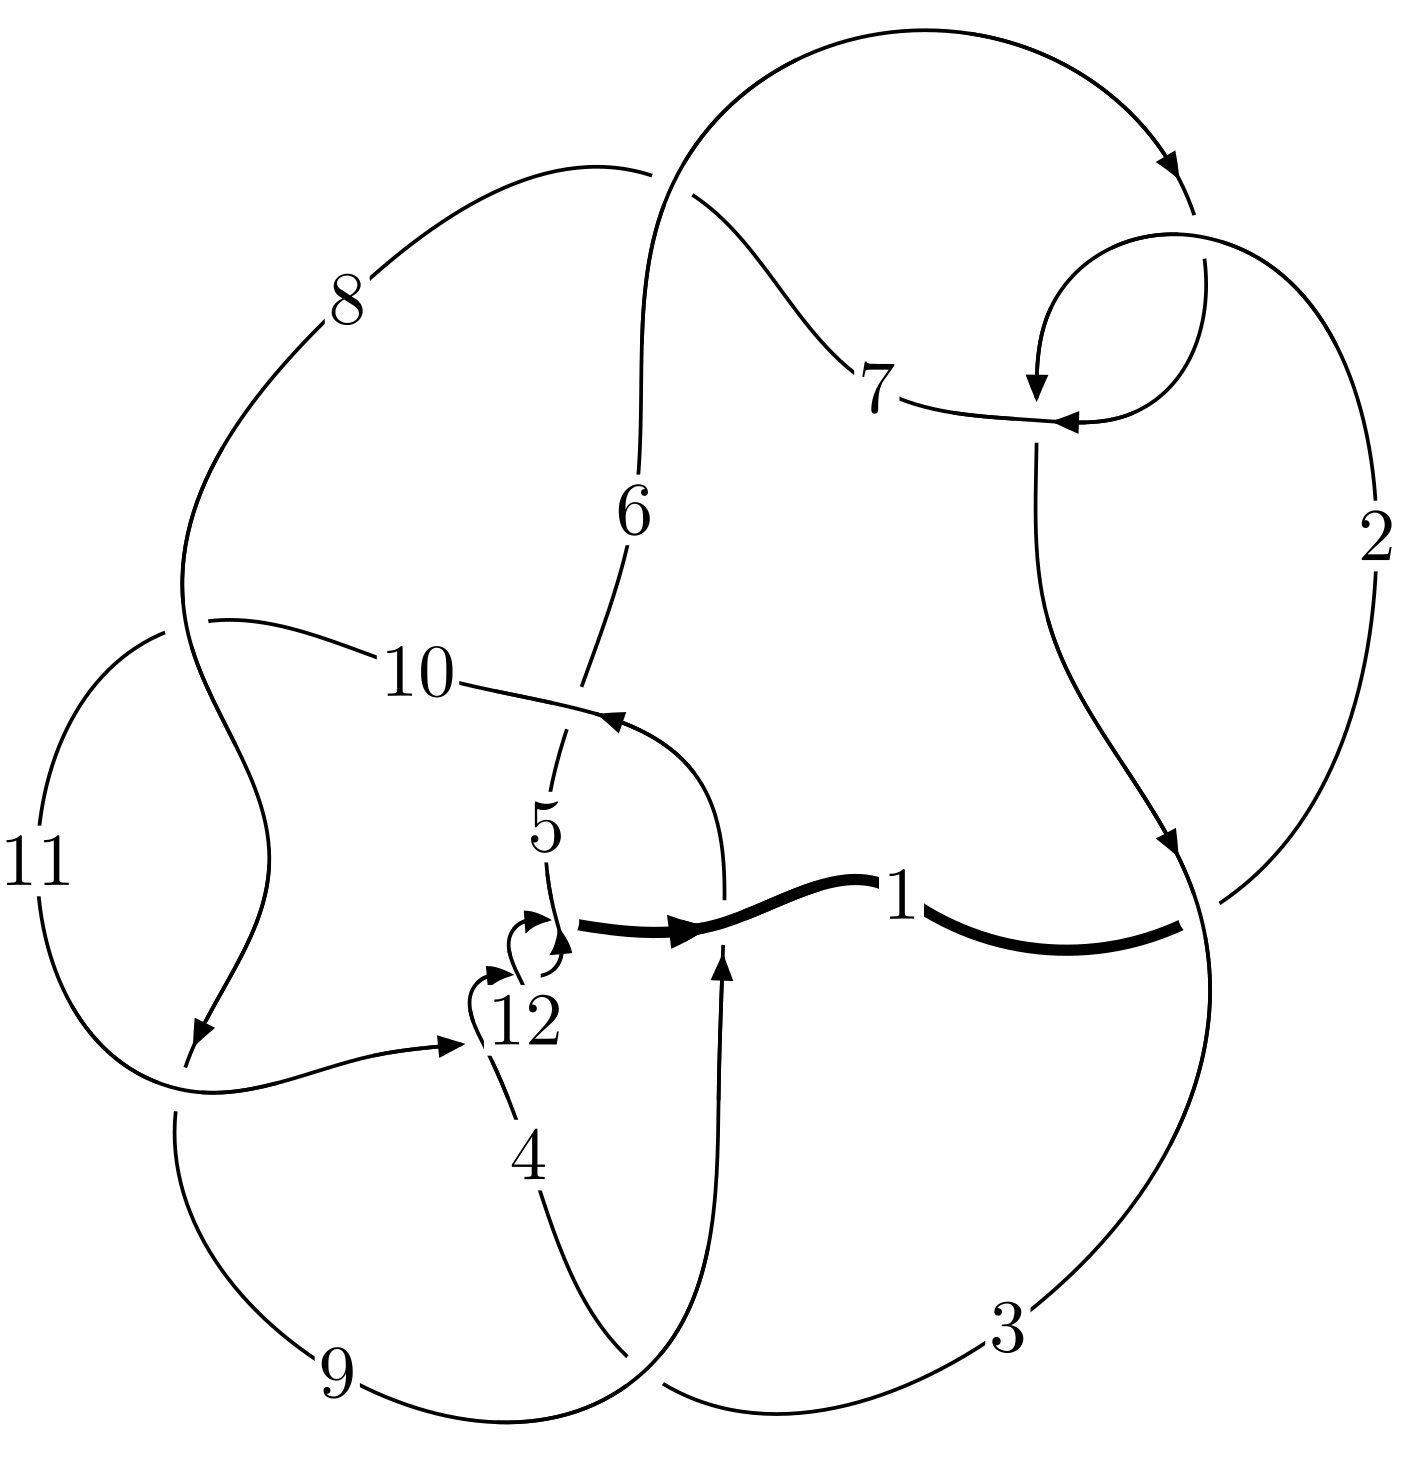
\includegraphics[width=112pt]{../../../GIT/diagram.site/Diagrams/png/1406_12a_0605.png}\\
\ \ \ A knot diagram\footnotemark}&
\allowdisplaybreaks
\textbf{Linearized knot diagam} \\
\cline{2-2}
 &
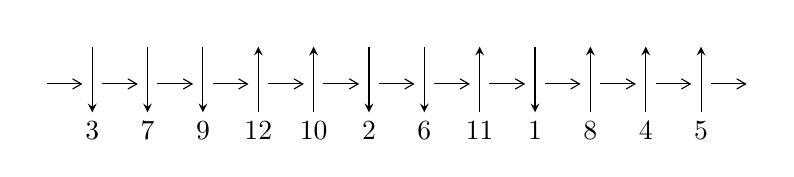
\begin{tikzpicture}[x=20pt, y=17pt]
	% nodes
	\node (C0) at (0, 0) {};
	\node (C1) at (1, 0) {};
	\node (C1U) at (1, +1) {};
	\node (C1D) at (1, -1) {3};

	\node (C2) at (2, 0) {};
	\node (C2U) at (2, +1) {};
	\node (C2D) at (2, -1) {7};

	\node (C3) at (3, 0) {};
	\node (C3U) at (3, +1) {};
	\node (C3D) at (3, -1) {9};

	\node (C4) at (4, 0) {};
	\node (C4U) at (4, +1) {};
	\node (C4D) at (4, -1) {12};

	\node (C5) at (5, 0) {};
	\node (C5U) at (5, +1) {};
	\node (C5D) at (5, -1) {10};

	\node (C6) at (6, 0) {};
	\node (C6U) at (6, +1) {};
	\node (C6D) at (6, -1) {2};

	\node (C7) at (7, 0) {};
	\node (C7U) at (7, +1) {};
	\node (C7D) at (7, -1) {6};

	\node (C8) at (8, 0) {};
	\node (C8U) at (8, +1) {};
	\node (C8D) at (8, -1) {11};

	\node (C9) at (9, 0) {};
	\node (C9U) at (9, +1) {};
	\node (C9D) at (9, -1) {1};

	\node (C10) at (10, 0) {};
	\node (C10U) at (10, +1) {};
	\node (C10D) at (10, -1) {8};

	\node (C11) at (11, 0) {};
	\node (C11U) at (11, +1) {};
	\node (C11D) at (11, -1) {4};

	\node (C12) at (12, 0) {};
	\node (C12U) at (12, +1) {};
	\node (C12D) at (12, -1) {5};
	\node (C13) at (13, 0) {};

	% arrows
	\draw[->,>={angle 60}]
	(C0) edge (C1) (C1) edge (C2) (C2) edge (C3) (C3) edge (C4) (C4) edge (C5) (C5) edge (C6) (C6) edge (C7) (C7) edge (C8) (C8) edge (C9) (C9) edge (C10) (C10) edge (C11) (C11) edge (C12) (C12) edge (C13) ;	\draw[->,>=stealth]
	(C1U) edge (C1D) (C2U) edge (C2D) (C3U) edge (C3D) (C4D) edge (C4U) (C5D) edge (C5U) (C6U) edge (C6D) (C7U) edge (C7D) (C8D) edge (C8U) (C9U) edge (C9D) (C10D) edge (C10U) (C11D) edge (C11U) (C12D) edge (C12U) ;
	\end{tikzpicture} \\
\hhline{~~} \\& 
\textbf{Solving Sequence} \\ \cline{2-2} 
 &
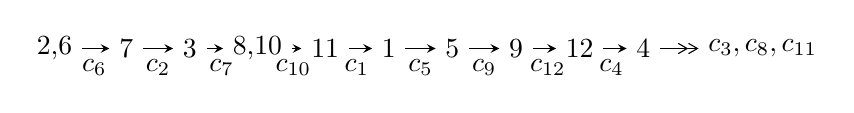
\begin{tikzpicture}[x=23pt, y=7pt]
	% node
	\node (A0) at (-1/8, 0) {2,6};
	\node (A1) at (1, 0) {7};
	\node (A2) at (2, 0) {3};
	\node (A3) at (49/16, 0) {8,10};
	\node (A4) at (33/8, 0) {11};
	\node (A5) at (41/8, 0) {1};
	\node (A6) at (49/8, 0) {5};
	\node (A7) at (57/8, 0) {9};
	\node (A8) at (65/8, 0) {12};
	\node (A9) at (73/8, 0) {4};
	\node (C1) at (1/2, -1) {$c_{6}$};
	\node (C2) at (3/2, -1) {$c_{2}$};
	\node (C3) at (5/2, -1) {$c_{7}$};
	\node (C4) at (29/8, -1) {$c_{10}$};
	\node (C5) at (37/8, -1) {$c_{1}$};
	\node (C6) at (45/8, -1) {$c_{5}$};
	\node (C7) at (53/8, -1) {$c_{9}$};
	\node (C8) at (61/8, -1) {$c_{12}$};
	\node (C9) at (69/8, -1) {$c_{4}$};
	\node (A10) at (11, 0) {$c_{3},c_{8},c_{11}$};

	% edge
	\draw[->,>=stealth]	
	(A0) edge (A1) (A1) edge (A2) (A2) edge (A3) (A3) edge (A4) (A4) edge (A5) (A5) edge (A6) (A6) edge (A7) (A7) edge (A8) (A8) edge (A9) ;
	\draw[->>,>={angle 60}]	
	(A9) edge (A10);
\end{tikzpicture} \\ 

\end{tabular} \\

\footnotetext{
The image of knot diagram is generated by the software ``\textbf{Draw programme}" developed by Andrew Bartholomew(\url{http://www.layer8.co.uk/maths/draw/index.htm\#Running-draw}), where we modified some parts for our purpose(\url{https://github.com/CATsTAILs/LinksPainter}).
}\phantom \\ \newline 
\centering \textbf{Ideals for irreducible components\footnotemark of $X_{\text{par}}$} 
 
\begin{align*}
I^u_{1}&=\langle 
-1.87845\times10^{64} u^{82}+1.27988\times10^{64} u^{81}+\cdots+2.92888\times10^{64} b-1.21244\times10^{64},\\
\phantom{I^u_{1}}&\phantom{= \langle  }-1.31389\times10^{63} u^{82}-1.25844\times10^{64} u^{81}+\cdots+2.92888\times10^{64} a-7.49424\times10^{64},\;u^{83}-2 u^{82}+\cdots+2 u-1\rangle \\
I^u_{2}&=\langle 
8 u^5+10 u^4-20 u^3-6 u^2+23 b+21 u-1,\;-5 u^5+11 u^4+u^3-2 u^2+23 a+7 u-8,\\
\phantom{I^u_{2}}&\phantom{= \langle  }u^6- u^5- u^4+2 u^3- u+1\rangle \\
\\
\end{align*}
\raggedright * 2 irreducible components of $\dim_{\mathbb{C}}=0$, with total 89 representations.\\
\footnotetext{All coefficients of polynomials are rational numbers. But the coefficients are sometimes approximated in decimal forms when there is not enough margin.}
\newpage
\renewcommand{\arraystretch}{1}
\centering \section*{I. $I^u_{1}= \langle -1.88\times10^{64} u^{82}+1.28\times10^{64} u^{81}+\cdots+2.93\times10^{64} b-1.21\times10^{64},\;-1.31\times10^{63} u^{82}-1.26\times10^{64} u^{81}+\cdots+2.93\times10^{64} a-7.49\times10^{64},\;u^{83}-2 u^{82}+\cdots+2 u-1 \rangle$}
\flushleft \textbf{(i) Arc colorings}\\
\begin{tabular}{m{7pt} m{180pt} m{7pt} m{180pt} }
\flushright $a_{2}=$&$\begin{pmatrix}0\\u\end{pmatrix}$ \\
\flushright $a_{6}=$&$\begin{pmatrix}1\\0\end{pmatrix}$ \\
\flushright $a_{7}=$&$\begin{pmatrix}1\\u^2\end{pmatrix}$ \\
\flushright $a_{3}=$&$\begin{pmatrix}- u\\- u^3+u\end{pmatrix}$ \\
\flushright $a_{8}=$&$\begin{pmatrix}- u^2+1\\u^2\end{pmatrix}$ \\
\flushright $a_{10}=$&$\begin{pmatrix}0.0448598 u^{82}+0.429664 u^{81}+\cdots-0.168626 u+2.55874\\0.641352 u^{82}-0.436985 u^{81}+\cdots-2.72216 u+0.413960\end{pmatrix}$ \\
\flushright $a_{11}=$&$\begin{pmatrix}0.0314267 u^{82}+0.354611 u^{81}+\cdots-0.923848 u+1.65310\\0.640827 u^{82}-0.379524 u^{81}+\cdots-2.64509 u+0.368450\end{pmatrix}$ \\
\flushright $a_{1}=$&$\begin{pmatrix}u^3\\u^5- u^3+u\end{pmatrix}$ \\
\flushright $a_{5}=$&$\begin{pmatrix}1.40123 u^{82}-2.52242 u^{81}+\cdots-2.31312 u+0.870884\\1.07497 u^{82}-1.14368 u^{81}+\cdots+2.45617 u+0.923234\end{pmatrix}$ \\
\flushright $a_{9}=$&$\begin{pmatrix}-0.000305313 u^{82}+0.492328 u^{81}+\cdots-0.144340 u+2.50567\\0.594051 u^{82}-0.368881 u^{81}+\cdots-2.46994 u+0.309558\end{pmatrix}$ \\
\flushright $a_{12}=$&$\begin{pmatrix}1.27948 u^{82}-1.88951 u^{81}+\cdots-2.58516 u+1.03474\\1.29851 u^{82}-1.69376 u^{81}+\cdots+1.45034 u+1.55967\end{pmatrix}$ \\
\flushright $a_{4}=$&$\begin{pmatrix}-1.24128 u^{82}+0.934848 u^{81}+\cdots-0.924884 u-1.12049\\-1.26658 u^{82}+1.49098 u^{81}+\cdots+5.74887 u-2.52264\end{pmatrix}$\\&\end{tabular}
\flushleft \textbf{(ii) Obstruction class $= -1$}\\~\\
\flushleft \textbf{(iii) Cusp Shapes $= -5.63470 u^{82}+9.65125 u^{81}+\cdots-3.31630 u-0.497855$}\\~\\
\newpage\renewcommand{\arraystretch}{1}
\flushleft \textbf{(iv) u-Polynomials at the component}\newline \\
\begin{tabular}{m{50pt}|m{274pt}}
Crossings & \hspace{64pt}u-Polynomials at each crossing \\
\hline $$\begin{aligned}c_{1},c_{7}\end{aligned}$$&$\begin{aligned}
&u^{83}+24 u^{82}+\cdots+8 u+1
\end{aligned}$\\
\hline $$\begin{aligned}c_{2},c_{6}\end{aligned}$$&$\begin{aligned}
&u^{83}-2 u^{82}+\cdots+2 u-1
\end{aligned}$\\
\hline $$\begin{aligned}c_{3}\end{aligned}$$&$\begin{aligned}
&23(23 u^{83}-133 u^{82}+\cdots+1.50077\times10^{7} u-1502291)
\end{aligned}$\\
\hline $$\begin{aligned}c_{4},c_{11},c_{12}\end{aligned}$$&$\begin{aligned}
&u^{83}-2 u^{82}+\cdots-4 u^2+1
\end{aligned}$\\
\hline $$\begin{aligned}c_{5}\end{aligned}$$&$\begin{aligned}
&23(23 u^{83}+64 u^{82}+\cdots+8416615 u+1304033)
\end{aligned}$\\
\hline $$\begin{aligned}c_{8},c_{10}\end{aligned}$$&$\begin{aligned}
&u^{83}+7 u^{82}+\cdots-1641 u-529
\end{aligned}$\\
\hline $$\begin{aligned}c_{9}\end{aligned}$$&$\begin{aligned}
&u^{83}+7 u^{82}+\cdots-69184 u+33856
\end{aligned}$\\
\hline
\end{tabular}\\~\\
\newpage\renewcommand{\arraystretch}{1}
\flushleft \textbf{(v) Riley Polynomials at the component}\newline \\
\begin{tabular}{m{50pt}|m{274pt}}
Crossings & \hspace{64pt}Riley Polynomials at each crossing \\
\hline $$\begin{aligned}c_{1},c_{7}\end{aligned}$$&$\begin{aligned}
&y^{83}+72 y^{82}+\cdots+44 y-1
\end{aligned}$\\
\hline $$\begin{aligned}c_{2},c_{6}\end{aligned}$$&$\begin{aligned}
&y^{83}-24 y^{82}+\cdots+8 y-1
\end{aligned}$\\
\hline $$\begin{aligned}c_{3}\end{aligned}$$&$\begin{aligned}
&529\\
&\cdot(529 y^{83}+28081 y^{82}+\cdots+38188375604614 y-2256878248681)
\end{aligned}$\\
\hline $$\begin{aligned}c_{4},c_{11},c_{12}\end{aligned}$$&$\begin{aligned}
&y^{83}-84 y^{82}+\cdots+8 y-1
\end{aligned}$\\
\hline $$\begin{aligned}c_{5}\end{aligned}$$&$\begin{aligned}
&529\\
&\cdot(529 y^{83}-32708 y^{82}+\cdots+39172776651029 y-1700502065089)
\end{aligned}$\\
\hline $$\begin{aligned}c_{8},c_{10}\end{aligned}$$&$\begin{aligned}
&y^{83}-75 y^{82}+\cdots+5875345 y-279841
\end{aligned}$\\
\hline $$\begin{aligned}c_{9}\end{aligned}$$&$\begin{aligned}
&y^{83}+39 y^{82}+\cdots-8242446336 y-1146228736
\end{aligned}$\\
\hline
\end{tabular}\\~\\
\newpage\flushleft \textbf{(vi) Complex Volumes and Cusp Shapes}
$$\begin{array}{c|c|c}  
\text{Solutions to }I^u_{1}& \I (\text{vol} + \sqrt{-1}CS) & \text{Cusp shape}\\
 \hline 
\begin{aligned}
u &= -0.889482 + 0.456836 I \\
a &= \phantom{-}0.534958 - 0.131930 I \\
b &= \phantom{-}0.104167 - 0.719375 I\end{aligned}
 & -1.41772 + 1.74895 I & \phantom{-0.000000 } 0 \\ \hline\begin{aligned}
u &= -0.889482 - 0.456836 I \\
a &= \phantom{-}0.534958 + 0.131930 I \\
b &= \phantom{-}0.104167 + 0.719375 I\end{aligned}
 & -1.41772 - 1.74895 I & \phantom{-0.000000 } 0 \\ \hline\begin{aligned}
u &= -0.935965 + 0.259286 I \\
a &= -1.04483 + 1.50530 I \\
b &= \phantom{-}0.900121 + 0.852842 I\end{aligned}
 & \phantom{-}3.42942 + 5.61464 I & \phantom{-0.000000 } 0. - 7.27404 I \\ \hline\begin{aligned}
u &= -0.935965 - 0.259286 I \\
a &= -1.04483 - 1.50530 I \\
b &= \phantom{-}0.900121 - 0.852842 I\end{aligned}
 & \phantom{-}3.42942 - 5.61464 I & \phantom{-0.000000 -}0. + 7.27404 I \\ \hline\begin{aligned}
u &= \phantom{-}0.941175 + 0.204587 I \\
a &= -0.721363 - 0.988163 I \\
b &= \phantom{-}0.592450 - 0.675808 I\end{aligned}
 & -2.60762 - 3.23702 I & -5.49466 + 7.80005 I \\ \hline\begin{aligned}
u &= \phantom{-}0.941175 - 0.204587 I \\
a &= -0.721363 + 0.988163 I \\
b &= \phantom{-}0.592450 + 0.675808 I\end{aligned}
 & -2.60762 + 3.23702 I & -5.49466 - 7.80005 I \\ \hline\begin{aligned}
u &= -0.953043 + 0.078413 I \\
a &= -0.334788 + 0.276834 I \\
b &= \phantom{-}0.331892 + 0.225291 I\end{aligned}
 & -1.83683 + 0.10839 I & -5.40972 + 0. I\phantom{ +0.000000I} \\ \hline\begin{aligned}
u &= -0.953043 - 0.078413 I \\
a &= -0.334788 - 0.276834 I \\
b &= \phantom{-}0.331892 - 0.225291 I\end{aligned}
 & -1.83683 - 0.10839 I & -5.40972 + 0. I\phantom{ +0.000000I} \\ \hline\begin{aligned}
u &= \phantom{-}0.849141 + 0.242956 I \\
a &= \phantom{-}1.018340 - 0.060762 I \\
b &= \phantom{-}0.905830 + 0.798266 I\end{aligned}
 & \phantom{-}3.46734 + 0.71154 I & -0.47127 + 2.15369 I \\ \hline\begin{aligned}
u &= \phantom{-}0.849141 - 0.242956 I \\
a &= \phantom{-}1.018340 + 0.060762 I \\
b &= \phantom{-}0.905830 - 0.798266 I\end{aligned}
 & \phantom{-}3.46734 - 0.71154 I & -0.47127 - 2.15369 I\\
 \hline 
 \end{array}$$\newpage$$\begin{array}{c|c|c}  
\text{Solutions to }I^u_{1}& \I (\text{vol} + \sqrt{-1}CS) & \text{Cusp shape}\\
 \hline 
\begin{aligned}
u &= \phantom{-}0.816703 + 0.768943 I \\
a &= \phantom{-}1.75089 + 0.20685 I \\
b &= -1.082510 + 0.403406 I\end{aligned}
 & \phantom{-}3.52701 - 1.42228 I & \phantom{-0.000000 } 0 \\ \hline\begin{aligned}
u &= \phantom{-}0.816703 - 0.768943 I \\
a &= \phantom{-}1.75089 - 0.20685 I \\
b &= -1.082510 - 0.403406 I\end{aligned}
 & \phantom{-}3.52701 + 1.42228 I & \phantom{-0.000000 } 0 \\ \hline\begin{aligned}
u &= -0.835455 + 0.753520 I \\
a &= \phantom{-}3.50927 + 0.93237 I \\
b &= -1.97135 - 2.14558 I\end{aligned}
 & \phantom{-}9.03093 + 2.89498 I & \phantom{-0.000000 } 0 \\ \hline\begin{aligned}
u &= -0.835455 - 0.753520 I \\
a &= \phantom{-}3.50927 - 0.93237 I \\
b &= -1.97135 + 2.14558 I\end{aligned}
 & \phantom{-}9.03093 - 2.89498 I & \phantom{-0.000000 } 0 \\ \hline\begin{aligned}
u &= -0.802716 + 0.802162 I \\
a &= \phantom{-}1.54959 - 0.71704 I \\
b &= -0.933558 + 0.245697 I\end{aligned}
 & \phantom{-}3.74533 - 1.60662 I & \phantom{-0.000000 } 0 \\ \hline\begin{aligned}
u &= -0.802716 - 0.802162 I \\
a &= \phantom{-}1.54959 + 0.71704 I \\
b &= -0.933558 - 0.245697 I\end{aligned}
 & \phantom{-}3.74533 + 1.60662 I & \phantom{-0.000000 } 0 \\ \hline\begin{aligned}
u &= \phantom{-}0.027665 + 0.862785 I \\
a &= -0.867205 - 0.219871 I \\
b &= \phantom{-}1.133800 + 0.169437 I\end{aligned}
 & \phantom{-}4.74686 + 2.93300 I & \phantom{-}8.76121 - 3.91326 I \\ \hline\begin{aligned}
u &= \phantom{-}0.027665 - 0.862785 I \\
a &= -0.867205 + 0.219871 I \\
b &= \phantom{-}1.133800 - 0.169437 I\end{aligned}
 & \phantom{-}4.74686 - 2.93300 I & \phantom{-}8.76121 + 3.91326 I \\ \hline\begin{aligned}
u &= -1.105370 + 0.315329 I \\
a &= \phantom{-}0.014499 - 1.098310 I \\
b &= -1.29278 - 0.74240 I\end{aligned}
 & \phantom{-}8.45345 + 11.00130 I & \phantom{-0.000000 } 0 \\ \hline\begin{aligned}
u &= -1.105370 - 0.315329 I \\
a &= \phantom{-}0.014499 + 1.098310 I \\
b &= -1.29278 + 0.74240 I\end{aligned}
 & \phantom{-}8.45345 - 11.00130 I & \phantom{-0.000000 } 0\\
 \hline 
 \end{array}$$\newpage$$\begin{array}{c|c|c}  
\text{Solutions to }I^u_{1}& \I (\text{vol} + \sqrt{-1}CS) & \text{Cusp shape}\\
 \hline 
\begin{aligned}
u &= \phantom{-}0.807856 + 0.824094 I \\
a &= \phantom{-}1.75320 + 0.96864 I \\
b &= -1.040670 - 0.534905 I\end{aligned}
 & \phantom{-}10.24590 + 3.75990 I & \phantom{-0.000000 } 0 \\ \hline\begin{aligned}
u &= \phantom{-}0.807856 - 0.824094 I \\
a &= \phantom{-}1.75320 - 0.96864 I \\
b &= -1.040670 + 0.534905 I\end{aligned}
 & \phantom{-}10.24590 - 3.75990 I & \phantom{-0.000000 } 0 \\ \hline\begin{aligned}
u &= \phantom{-}0.834963\phantom{ +0.000000I} \\
a &= \phantom{-}3.68259\phantom{ +0.000000I} \\
b &= \phantom{-}4.90505\phantom{ +0.000000I}\end{aligned}
 & \phantom{-}5.65010\phantom{ +0.000000I} & -26.1310\phantom{ +0.000000I} \\ \hline\begin{aligned}
u &= \phantom{-}0.515647 + 0.654524 I \\
a &= \phantom{-}0.414145 - 0.145965 I \\
b &= \phantom{-}0.261027 + 0.341321 I\end{aligned}
 & \phantom{-}2.62411 + 0.87584 I & \phantom{-}0.235931 + 0.049304 I \\ \hline\begin{aligned}
u &= \phantom{-}0.515647 - 0.654524 I \\
a &= \phantom{-}0.414145 + 0.145965 I \\
b &= \phantom{-}0.261027 - 0.341321 I\end{aligned}
 & \phantom{-}2.62411 - 0.87584 I & \phantom{-}0.235931 - 0.049304 I \\ \hline\begin{aligned}
u &= \phantom{-}1.140330 + 0.259412 I \\
a &= -0.706300 + 0.694710 I \\
b &= -1.008980 - 0.277275 I\end{aligned}
 & \phantom{-}8.05514 + 3.48111 I & \phantom{-0.000000 } 0 \\ \hline\begin{aligned}
u &= \phantom{-}1.140330 - 0.259412 I \\
a &= -0.706300 - 0.694710 I \\
b &= -1.008980 + 0.277275 I\end{aligned}
 & \phantom{-}8.05514 - 3.48111 I & \phantom{-0.000000 } 0 \\ \hline\begin{aligned}
u &= -0.033678 + 0.823507 I \\
a &= -1.127770 + 0.564262 I \\
b &= \phantom{-}1.337490 - 0.420345 I\end{aligned}
 & \phantom{-}12.04910 - 7.13476 I & \phantom{-}9.25485 + 4.05212 I \\ \hline\begin{aligned}
u &= -0.033678 - 0.823507 I \\
a &= -1.127770 - 0.564262 I \\
b &= \phantom{-}1.337490 + 0.420345 I\end{aligned}
 & \phantom{-}12.04910 + 7.13476 I & \phantom{-}9.25485 - 4.05212 I \\ \hline\begin{aligned}
u &= \phantom{-}0.884797 + 0.775848 I \\
a &= -1.77395 + 1.63904 I \\
b &= -0.07694 - 2.70204 I\end{aligned}
 & \phantom{-}5.37866 - 2.92461 I & \phantom{-0.000000 } 0\\
 \hline 
 \end{array}$$\newpage$$\begin{array}{c|c|c}  
\text{Solutions to }I^u_{1}& \I (\text{vol} + \sqrt{-1}CS) & \text{Cusp shape}\\
 \hline 
\begin{aligned}
u &= \phantom{-}0.884797 - 0.775848 I \\
a &= -1.77395 - 1.63904 I \\
b &= -0.07694 + 2.70204 I\end{aligned}
 & \phantom{-}5.37866 + 2.92461 I & \phantom{-0.000000 } 0 \\ \hline\begin{aligned}
u &= \phantom{-}1.127720 + 0.337758 I \\
a &= -0.044991 + 0.823378 I \\
b &= -0.960090 + 0.541916 I\end{aligned}
 & \phantom{-}1.04660 - 7.01205 I & \phantom{-0.000000 } 0 \\ \hline\begin{aligned}
u &= \phantom{-}1.127720 - 0.337758 I \\
a &= -0.044991 - 0.823378 I \\
b &= -0.960090 - 0.541916 I\end{aligned}
 & \phantom{-}1.04660 + 7.01205 I & \phantom{-0.000000 } 0 \\ \hline\begin{aligned}
u &= -0.732275 + 0.922468 I \\
a &= -1.009770 + 0.052035 I \\
b &= \phantom{-}1.227170 - 0.199103 I\end{aligned}
 & \phantom{-}16.1676 + 3.4606 I & \phantom{-0.000000 } 0 \\ \hline\begin{aligned}
u &= -0.732275 - 0.922468 I \\
a &= -1.009770 - 0.052035 I \\
b &= \phantom{-}1.227170 + 0.199103 I\end{aligned}
 & \phantom{-}16.1676 - 3.4606 I & \phantom{-0.000000 } 0 \\ \hline\begin{aligned}
u &= \phantom{-}0.754229 + 0.905051 I \\
a &= -1.52604 - 0.95557 I \\
b &= \phantom{-}1.72976 + 0.81123 I\end{aligned}
 & \phantom{-}16.6561 + 10.4380 I & \phantom{-0.000000 } 0 \\ \hline\begin{aligned}
u &= \phantom{-}0.754229 - 0.905051 I \\
a &= -1.52604 + 0.95557 I \\
b &= \phantom{-}1.72976 - 0.81123 I\end{aligned}
 & \phantom{-}16.6561 - 10.4380 I & \phantom{-0.000000 } 0 \\ \hline\begin{aligned}
u &= -0.867281 + 0.802103 I \\
a &= \phantom{-}0.810453 - 0.423035 I \\
b &= -1.014500 + 0.771217 I\end{aligned}
 & \phantom{-}7.30880 + 1.13595 I & \phantom{-0.000000 } 0 \\ \hline\begin{aligned}
u &= -0.867281 - 0.802103 I \\
a &= \phantom{-}0.810453 + 0.423035 I \\
b &= -1.014500 - 0.771217 I\end{aligned}
 & \phantom{-}7.30880 - 1.13595 I & \phantom{-0.000000 } 0 \\ \hline\begin{aligned}
u &= -0.917071 + 0.745377 I \\
a &= -0.69179 + 3.01817 I \\
b &= \phantom{-}2.07340 - 1.42336 I\end{aligned}
 & \phantom{-}8.78061 + 2.79415 I & \phantom{-0.000000 } 0\\
 \hline 
 \end{array}$$\newpage$$\begin{array}{c|c|c}  
\text{Solutions to }I^u_{1}& \I (\text{vol} + \sqrt{-1}CS) & \text{Cusp shape}\\
 \hline 
\begin{aligned}
u &= -0.917071 - 0.745377 I \\
a &= -0.69179 - 3.01817 I \\
b &= \phantom{-}2.07340 + 1.42336 I\end{aligned}
 & \phantom{-}8.78061 - 2.79415 I & \phantom{-0.000000 } 0 \\ \hline\begin{aligned}
u &= -0.731443 + 0.355891 I \\
a &= \phantom{-}0.99738 + 2.75342 I \\
b &= \phantom{-}0.486901 - 0.522296 I\end{aligned}
 & \phantom{-}7.80848 + 3.23449 I & \phantom{-}6.54878 - 6.03977 I \\ \hline\begin{aligned}
u &= -0.731443 - 0.355891 I \\
a &= \phantom{-}0.99738 - 2.75342 I \\
b &= \phantom{-}0.486901 + 0.522296 I\end{aligned}
 & \phantom{-}7.80848 - 3.23449 I & \phantom{-}6.54878 + 6.03977 I \\ \hline\begin{aligned}
u &= -0.757746 + 0.913416 I \\
a &= -1.21392 + 0.81604 I \\
b &= \phantom{-}1.48040 - 0.75317 I\end{aligned}
 & \phantom{-}9.48311 - 6.48346 I & \phantom{-0.000000 } 0 \\ \hline\begin{aligned}
u &= -0.757746 - 0.913416 I \\
a &= -1.21392 - 0.81604 I \\
b &= \phantom{-}1.48040 + 0.75317 I\end{aligned}
 & \phantom{-}9.48311 + 6.48346 I & \phantom{-0.000000 } 0 \\ \hline\begin{aligned}
u &= \phantom{-}1.034880 + 0.585496 I \\
a &= \phantom{-}0.099302 + 0.223114 I \\
b &= -0.135254 + 0.437889 I\end{aligned}
 & \phantom{-}1.11865 - 5.75066 I & \phantom{-0.000000 } 0 \\ \hline\begin{aligned}
u &= \phantom{-}1.034880 - 0.585496 I \\
a &= \phantom{-}0.099302 - 0.223114 I \\
b &= -0.135254 - 0.437889 I\end{aligned}
 & \phantom{-}1.11865 + 5.75066 I & \phantom{-0.000000 } 0 \\ \hline\begin{aligned}
u &= \phantom{-}0.750775 + 0.926710 I \\
a &= -0.987309 - 0.492800 I \\
b &= \phantom{-}1.262870 + 0.541456 I\end{aligned}
 & \phantom{-}9.20226 + 0.93743 I & \phantom{-0.000000 } 0 \\ \hline\begin{aligned}
u &= \phantom{-}0.750775 - 0.926710 I \\
a &= -0.987309 + 0.492800 I \\
b &= \phantom{-}1.262870 - 0.541456 I\end{aligned}
 & \phantom{-}9.20226 - 0.93743 I & \phantom{-0.000000 } 0 \\ \hline\begin{aligned}
u &= \phantom{-}0.870208 + 0.820915 I \\
a &= \phantom{-}1.250600 - 0.413944 I \\
b &= -0.905844 - 0.271334 I\end{aligned}
 & \phantom{-}14.3924 - 0.4286 I & \phantom{-0.000000 } 0\\
 \hline 
 \end{array}$$\newpage$$\begin{array}{c|c|c}  
\text{Solutions to }I^u_{1}& \I (\text{vol} + \sqrt{-1}CS) & \text{Cusp shape}\\
 \hline 
\begin{aligned}
u &= \phantom{-}0.870208 - 0.820915 I \\
a &= \phantom{-}1.250600 + 0.413944 I \\
b &= -0.905844 + 0.271334 I\end{aligned}
 & \phantom{-}14.3924 + 0.4286 I & \phantom{-0.000000 } 0 \\ \hline\begin{aligned}
u &= \phantom{-}0.937268 + 0.745740 I \\
a &= -1.19353 - 1.12183 I \\
b &= \phantom{-}1.122130 + 0.134120 I\end{aligned}
 & \phantom{-}3.15571 - 4.31418 I & \phantom{-0.000000 } 0 \\ \hline\begin{aligned}
u &= \phantom{-}0.937268 - 0.745740 I \\
a &= -1.19353 + 1.12183 I \\
b &= \phantom{-}1.122130 - 0.134120 I\end{aligned}
 & \phantom{-}3.15571 + 4.31418 I & \phantom{-0.000000 } 0 \\ \hline\begin{aligned}
u &= -0.909622 + 0.790683 I \\
a &= -1.56898 + 0.84569 I \\
b &= \phantom{-}0.853137 + 0.850342 I\end{aligned}
 & \phantom{-}7.17818 + 4.83871 I & \phantom{-0.000000 } 0 \\ \hline\begin{aligned}
u &= -0.909622 - 0.790683 I \\
a &= -1.56898 - 0.84569 I \\
b &= \phantom{-}0.853137 - 0.850342 I\end{aligned}
 & \phantom{-}7.17818 - 4.83871 I & \phantom{-0.000000 } 0 \\ \hline\begin{aligned}
u &= -1.178820 + 0.299322 I \\
a &= -0.340622 - 0.623463 I \\
b &= -0.844509 - 0.119752 I\end{aligned}
 & \phantom{-}0.662850 + 1.033910 I & \phantom{-0.000000 } 0 \\ \hline\begin{aligned}
u &= -1.178820 - 0.299322 I \\
a &= -0.340622 + 0.623463 I \\
b &= -0.844509 + 0.119752 I\end{aligned}
 & \phantom{-}0.662850 - 1.033910 I & \phantom{-0.000000 } 0 \\ \hline\begin{aligned}
u &= \phantom{-}0.916556 + 0.806377 I \\
a &= -1.28781 - 1.55467 I \\
b &= \phantom{-}0.779647 - 0.298397 I\end{aligned}
 & \phantom{-}14.2487 - 5.6526 I & \phantom{-0.000000 } 0 \\ \hline\begin{aligned}
u &= \phantom{-}0.916556 - 0.806377 I \\
a &= -1.28781 + 1.55467 I \\
b &= \phantom{-}0.779647 + 0.298397 I\end{aligned}
 & \phantom{-}14.2487 + 5.6526 I & \phantom{-0.000000 } 0 \\ \hline\begin{aligned}
u &= -0.955332 + 0.764210 I \\
a &= -1.80085 + 0.64179 I \\
b &= \phantom{-}1.017290 + 0.386028 I\end{aligned}
 & \phantom{-}3.27752 + 7.49822 I & \phantom{-0.000000 } 0\\
 \hline 
 \end{array}$$\newpage$$\begin{array}{c|c|c}  
\text{Solutions to }I^u_{1}& \I (\text{vol} + \sqrt{-1}CS) & \text{Cusp shape}\\
 \hline 
\begin{aligned}
u &= -0.955332 - 0.764210 I \\
a &= -1.80085 - 0.64179 I \\
b &= \phantom{-}1.017290 - 0.386028 I\end{aligned}
 & \phantom{-}3.27752 - 7.49822 I & \phantom{-0.000000 } 0 \\ \hline\begin{aligned}
u &= \phantom{-}0.731306 + 0.256638 I \\
a &= \phantom{-}0.78032 - 2.04828 I \\
b &= \phantom{-}0.327098 - 0.173264 I\end{aligned}
 & \phantom{-}1.33574 - 2.24205 I & \phantom{-}4.43086 + 8.82898 I \\ \hline\begin{aligned}
u &= \phantom{-}0.731306 - 0.256638 I \\
a &= \phantom{-}0.78032 + 2.04828 I \\
b &= \phantom{-}0.327098 + 0.173264 I\end{aligned}
 & \phantom{-}1.33574 + 2.24205 I & \phantom{-}4.43086 - 8.82898 I \\ \hline\begin{aligned}
u &= \phantom{-}0.960254 + 0.779064 I \\
a &= -2.28212 - 0.60862 I \\
b &= \phantom{-}1.118770 - 0.610843 I\end{aligned}
 & \phantom{-}9.77627 - 9.76260 I & \phantom{-0.000000 } 0 \\ \hline\begin{aligned}
u &= \phantom{-}0.960254 - 0.779064 I \\
a &= -2.28212 + 0.60862 I \\
b &= \phantom{-}1.118770 + 0.610843 I\end{aligned}
 & \phantom{-}9.77627 + 9.76260 I & \phantom{-0.000000 } 0 \\ \hline\begin{aligned}
u &= -0.730104 + 0.111818 I \\
a &= \phantom{-}0.68230 + 2.05904 I \\
b &= \phantom{-}0.07317 + 1.79240 I\end{aligned}
 & \phantom{-}0.491768 + 0.412209 I & \phantom{-}3.6447 + 16.5037 I \\ \hline\begin{aligned}
u &= -0.730104 - 0.111818 I \\
a &= \phantom{-}0.68230 - 2.05904 I \\
b &= \phantom{-}0.07317 - 1.79240 I\end{aligned}
 & \phantom{-}0.491768 - 0.412209 I & \phantom{-}3.6447 - 16.5037 I \\ \hline\begin{aligned}
u &= \phantom{-}1.024460 + 0.793490 I \\
a &= \phantom{-}2.08009 + 1.18604 I \\
b &= -1.72181 + 0.93118 I\end{aligned}
 & \phantom{-}15.8084 - 16.7169 I & \phantom{-0.000000 } 0 \\ \hline\begin{aligned}
u &= \phantom{-}1.024460 - 0.793490 I \\
a &= \phantom{-}2.08009 - 1.18604 I \\
b &= -1.72181 - 0.93118 I\end{aligned}
 & \phantom{-}15.8084 + 16.7169 I & \phantom{-0.000000 } 0 \\ \hline\begin{aligned}
u &= -1.026430 + 0.799370 I \\
a &= \phantom{-}1.78257 - 0.95986 I \\
b &= -1.44862 - 0.89101 I\end{aligned}
 & \phantom{-}8.6384 + 12.8059 I & \phantom{-0.000000 } 0\\
 \hline 
 \end{array}$$\newpage$$\begin{array}{c|c|c}  
\text{Solutions to }I^u_{1}& \I (\text{vol} + \sqrt{-1}CS) & \text{Cusp shape}\\
 \hline 
\begin{aligned}
u &= -1.026430 - 0.799370 I \\
a &= \phantom{-}1.78257 + 0.95986 I \\
b &= -1.44862 + 0.89101 I\end{aligned}
 & \phantom{-}8.6384 - 12.8059 I & \phantom{-0.000000 } 0 \\ \hline\begin{aligned}
u &= \phantom{-}1.035970 + 0.804028 I \\
a &= \phantom{-}1.33910 + 0.89568 I \\
b &= -1.187330 + 0.688916 I\end{aligned}
 & \phantom{-}8.30656 - 7.31250 I & \phantom{-0.000000 } 0 \\ \hline\begin{aligned}
u &= \phantom{-}1.035970 - 0.804028 I \\
a &= \phantom{-}1.33910 - 0.89568 I \\
b &= -1.187330 - 0.688916 I\end{aligned}
 & \phantom{-}8.30656 + 7.31250 I & \phantom{-0.000000 } 0 \\ \hline\begin{aligned}
u &= -1.046110 + 0.792804 I \\
a &= \phantom{-}0.87735 - 1.17014 I \\
b &= -1.099350 - 0.306452 I\end{aligned}
 & \phantom{-}15.1856 + 2.8676 I & \phantom{-0.000000 } 0 \\ \hline\begin{aligned}
u &= -1.046110 - 0.792804 I \\
a &= \phantom{-}0.87735 + 1.17014 I \\
b &= -1.099350 + 0.306452 I\end{aligned}
 & \phantom{-}15.1856 - 2.8676 I & \phantom{-0.000000 } 0 \\ \hline\begin{aligned}
u &= -0.387829 + 0.383433 I \\
a &= \phantom{-}2.84274 + 0.86881 I \\
b &= -1.325450 - 0.237969 I\end{aligned}
 & \phantom{-}8.75382 - 0.29598 I & \phantom{-}9.26455 - 1.68799 I \\ \hline\begin{aligned}
u &= -0.387829 - 0.383433 I \\
a &= \phantom{-}2.84274 - 0.86881 I \\
b &= -1.325450 + 0.237969 I\end{aligned}
 & \phantom{-}8.75382 + 0.29598 I & \phantom{-}9.26455 + 1.68799 I \\ \hline\begin{aligned}
u &= -0.056323 + 0.493607 I \\
a &= \phantom{-}1.90426 - 1.11553 I \\
b &= -0.725500 + 0.857677 I\end{aligned}
 & \phantom{-}5.99111 - 2.95551 I & \phantom{-}7.65900 + 2.93684 I \\ \hline\begin{aligned}
u &= -0.056323 - 0.493607 I \\
a &= \phantom{-}1.90426 + 1.11553 I \\
b &= -0.725500 - 0.857677 I\end{aligned}
 & \phantom{-}5.99111 + 2.95551 I & \phantom{-}7.65900 - 2.93684 I \\ \hline\begin{aligned}
u &= -0.047810 + 0.406306 I \\
a &= \phantom{-}1.37577 + 0.54247 I \\
b &= -0.346996 - 0.440258 I\end{aligned}
 & \phantom{-}0.164287 + 1.105020 I & \phantom{-}2.26614 - 6.04116 I\\
 \hline 
 \end{array}$$\newpage$$\begin{array}{c|c|c}  
\text{Solutions to }I^u_{1}& \I (\text{vol} + \sqrt{-1}CS) & \text{Cusp shape}\\
 \hline 
\begin{aligned}
u &= -0.047810 - 0.406306 I \\
a &= \phantom{-}1.37577 - 0.54247 I \\
b &= -0.346996 + 0.440258 I\end{aligned}
 & \phantom{-}0.164287 - 1.105020 I & \phantom{-}2.26614 + 6.04116 I \\ \hline\begin{aligned}
u &= \phantom{-}0.355483 + 0.185180 I \\
a &= \phantom{-}1.94592 - 0.44264 I \\
b &= -1.057690 + 0.002867 I\end{aligned}
 & \phantom{-}2.29106 + 0.03654 I & \phantom{-}6.03784 + 2.48416 I \\ \hline\begin{aligned}
u &= \phantom{-}0.355483 - 0.185180 I \\
a &= \phantom{-}1.94592 + 0.44264 I \\
b &= -1.057690 - 0.002867 I\end{aligned}
 & \phantom{-}2.29106 - 0.03654 I & \phantom{-}6.03784 - 2.48416 I\\
 \hline 
 \end{array}$$\newpage\newpage\renewcommand{\arraystretch}{1}
\centering \section*{II. $I^u_{2}= \langle 8 u^5+10 u^4-20 u^3-6 u^2+23 b+21 u-1,\;-5 u^5+11 u^4+u^3-2 u^2+23 a+7 u-8,\;u^6- u^5- u^4+2 u^3- u+1 \rangle$}
\flushleft \textbf{(i) Arc colorings}\\
\begin{tabular}{m{7pt} m{180pt} m{7pt} m{180pt} }
\flushright $a_{2}=$&$\begin{pmatrix}0\\u\end{pmatrix}$ \\
\flushright $a_{6}=$&$\begin{pmatrix}1\\0\end{pmatrix}$ \\
\flushright $a_{7}=$&$\begin{pmatrix}1\\u^2\end{pmatrix}$ \\
\flushright $a_{3}=$&$\begin{pmatrix}- u\\- u^3+u\end{pmatrix}$ \\
\flushright $a_{8}=$&$\begin{pmatrix}- u^2+1\\u^2\end{pmatrix}$ \\
\flushright $a_{10}=$&$\begin{pmatrix}0.217391 u^{5}-0.478261 u^{4}+\cdots-0.304348 u+0.347826\\-0.347826 u^{5}-0.434783 u^{4}+\cdots-0.913043 u+0.0434783\end{pmatrix}$ \\
\flushright $a_{11}=$&$\begin{pmatrix}0.217391 u^{5}-0.478261 u^{4}+\cdots-0.304348 u-0.652174\\-0.347826 u^{5}-0.434783 u^{4}+\cdots-0.913043 u+0.0434783\end{pmatrix}$ \\
\flushright $a_{1}=$&$\begin{pmatrix}u^3\\u^5- u^3+u\end{pmatrix}$ \\
\flushright $a_{5}=$&$\begin{pmatrix}0.0472590 u^{5}-0.364839 u^{4}+\cdots-0.283554 u+0.858223\\0.272212 u^{5}-0.181474 u^{4}+\cdots+0.366730 u+0.183365\end{pmatrix}$ \\
\flushright $a_{9}=$&$\begin{pmatrix}0.217391 u^{5}-0.478261 u^{4}+\cdots-0.304348 u+0.347826\\-0.347826 u^{5}-0.434783 u^{4}+\cdots-0.913043 u+0.0434783\end{pmatrix}$ \\
\flushright $a_{12}=$&$\begin{pmatrix}-0.676749 u^{5}-0.215501 u^{4}+\cdots-0.939509 u+0.0302457\\0.621928 u^{5}-0.0812854 u^{4}+\cdots+0.268431 u+0.134216\end{pmatrix}$ \\
\flushright $a_{4}=$&$\begin{pmatrix}-0.00378072 u^{5}-0.330813 u^{4}+\cdots-0.977316 u+0.0113422\\-0.141777 u^{5}+0.0945180 u^{4}+\cdots+0.850662 u+0.425331\end{pmatrix}$\\&\end{tabular}
\flushleft \textbf{(ii) Obstruction class $= 1$}\\~\\
\flushleft \textbf{(iii) Cusp Shapes $= -\frac{1101}{529} u^5+\frac{2321}{529} u^4+\frac{993}{529} u^3-\frac{3458}{529} u^2+\frac{2903}{529} u+\frac{4361}{529}$}\\~\\
\newpage\renewcommand{\arraystretch}{1}
\flushleft \textbf{(iv) u-Polynomials at the component}\newline \\
\begin{tabular}{m{50pt}|m{274pt}}
Crossings & \hspace{64pt}u-Polynomials at each crossing \\
\hline $$\begin{aligned}c_{1}\end{aligned}$$&$\begin{aligned}
&u^6-3 u^5+5 u^4-4 u^3+2 u^2- u+1
\end{aligned}$\\
\hline $$\begin{aligned}c_{2},c_{4}\end{aligned}$$&$\begin{aligned}
&u^6+u^5- u^4-2 u^3+u+1
\end{aligned}$\\
\hline $$\begin{aligned}c_{3}\end{aligned}$$&$\begin{aligned}
&23(23 u^6-18 u^5+25 u^4-8 u^3+7 u^2- u+1)
\end{aligned}$\\
\hline $$\begin{aligned}c_{5}\end{aligned}$$&$\begin{aligned}
&23(23 u^6-5 u^5-17 u^4+10 u^3+3 u^2-4 u+1)
\end{aligned}$\\
\hline $$\begin{aligned}c_{6},c_{11},c_{12}\end{aligned}$$&$\begin{aligned}
&u^6- u^5- u^4+2 u^3- u+1
\end{aligned}$\\
\hline $$\begin{aligned}c_{7}\end{aligned}$$&$\begin{aligned}
&u^6+3 u^5+5 u^4+4 u^3+2 u^2+u+1
\end{aligned}$\\
\hline $$\begin{aligned}c_{8}\end{aligned}$$&$\begin{aligned}
&(u+1)^6
\end{aligned}$\\
\hline $$\begin{aligned}c_{9}\end{aligned}$$&$\begin{aligned}
&u^6
\end{aligned}$\\
\hline $$\begin{aligned}c_{10}\end{aligned}$$&$\begin{aligned}
&(u-1)^6
\end{aligned}$\\
\hline
\end{tabular}\\~\\
\newpage\renewcommand{\arraystretch}{1}
\flushleft \textbf{(v) Riley Polynomials at the component}\newline \\
\begin{tabular}{m{50pt}|m{274pt}}
Crossings & \hspace{64pt}Riley Polynomials at each crossing \\
\hline $$\begin{aligned}c_{1},c_{7}\end{aligned}$$&$\begin{aligned}
&y^6+y^5+5 y^4+6 y^2+3 y+1
\end{aligned}$\\
\hline $$\begin{aligned}c_{2},c_{4},c_{6}\\c_{11},c_{12}\end{aligned}$$&$\begin{aligned}
&y^6-3 y^5+5 y^4-4 y^3+2 y^2- y+1
\end{aligned}$\\
\hline $$\begin{aligned}c_{3}\end{aligned}$$&$\begin{aligned}
&529(529 y^6+826 y^5+659 y^4+296 y^3+83 y^2+13 y+1)
\end{aligned}$\\
\hline $$\begin{aligned}c_{5}\end{aligned}$$&$\begin{aligned}
&529(529 y^6-807 y^5+527 y^4-196 y^3+55 y^2-10 y+1)
\end{aligned}$\\
\hline $$\begin{aligned}c_{8},c_{10}\end{aligned}$$&$\begin{aligned}
&(y-1)^6
\end{aligned}$\\
\hline $$\begin{aligned}c_{9}\end{aligned}$$&$\begin{aligned}
&y^6
\end{aligned}$\\
\hline
\end{tabular}\\~\\
\newpage\flushleft \textbf{(vi) Complex Volumes and Cusp Shapes}
$$\begin{array}{c|c|c}  
\text{Solutions to }I^u_{2}& \I (\text{vol} + \sqrt{-1}CS) & \text{Cusp shape}\\
 \hline 
\begin{aligned}
u &= -1.002190 + 0.295542 I \\
a &= \phantom{-}0.493592 + 0.608759 I \\
b &= \phantom{-}0.396884 + 0.370811 I\end{aligned}
 & -0.245672 + 0.924305 I & -2.14301 - 0.21731 I \\ \hline\begin{aligned}
u &= -1.002190 - 0.295542 I \\
a &= \phantom{-}0.493592 - 0.608759 I \\
b &= \phantom{-}0.396884 - 0.370811 I\end{aligned}
 & -0.245672 - 0.924305 I & -2.14301 + 0.21731 I \\ \hline\begin{aligned}
u &= \phantom{-}0.428243 + 0.664531 I \\
a &= \phantom{-}0.357844 - 0.079850 I \\
b &= -0.757689 - 0.164486 I\end{aligned}
 & \phantom{-}3.53554 + 0.92430 I & \phantom{-}10.05826 - 0.61014 I \\ \hline\begin{aligned}
u &= \phantom{-}0.428243 - 0.664531 I \\
a &= \phantom{-}0.357844 + 0.079850 I \\
b &= -0.757689 + 0.164486 I\end{aligned}
 & \phantom{-}3.53554 - 0.92430 I & \phantom{-}10.05826 + 0.61014 I \\ \hline\begin{aligned}
u &= \phantom{-}1.073950 + 0.558752 I \\
a &= \phantom{-}0.018129 - 0.725425 I \\
b &= \phantom{-}0.469501 - 0.157241 I\end{aligned}
 & \phantom{-}1.64493 - 5.69302 I & \phantom{-}9.84656 + 3.72057 I \\ \hline\begin{aligned}
u &= \phantom{-}1.073950 - 0.558752 I \\
a &= \phantom{-}0.018129 + 0.725425 I \\
b &= \phantom{-}0.469501 + 0.157241 I\end{aligned}
 & \phantom{-}1.64493 + 5.69302 I & \phantom{-}9.84656 - 3.72057 I\\
 \hline 
 \end{array}$$\newpage
\newpage\renewcommand{\arraystretch}{1}
\centering \section*{ III. u-Polynomials}
\begin{tabular}{m{50pt}|m{274pt}}
Crossings & \hspace{64pt}u-Polynomials at each crossing \\
\hline $$\begin{aligned}c_{1}\end{aligned}$$&$\begin{aligned}
&(u^6-3 u^5+5 u^4-4 u^3+2 u^2- u+1)(u^{83}+24 u^{82}+\cdots+8 u+1)
\end{aligned}$\\
\hline $$\begin{aligned}c_{2}\end{aligned}$$&$\begin{aligned}
&(u^6+u^5- u^4-2 u^3+u+1)(u^{83}-2 u^{82}+\cdots+2 u-1)
\end{aligned}$\\
\hline $$\begin{aligned}c_{3}\end{aligned}$$&$\begin{aligned}
&529(23 u^6-18 u^5+25 u^4-8 u^3+7 u^2- u+1)\\
&\cdot(23 u^{83}-133 u^{82}+\cdots+15007694 u-1502291)
\end{aligned}$\\
\hline $$\begin{aligned}c_{4}\end{aligned}$$&$\begin{aligned}
&(u^6+u^5- u^4-2 u^3+u+1)(u^{83}-2 u^{82}+\cdots-4 u^2+1)
\end{aligned}$\\
\hline $$\begin{aligned}c_{5}\end{aligned}$$&$\begin{aligned}
&529(23 u^6-5 u^5-17 u^4+10 u^3+3 u^2-4 u+1)\\
&\cdot(23 u^{83}+64 u^{82}+\cdots+8416615 u+1304033)
\end{aligned}$\\
\hline $$\begin{aligned}c_{6}\end{aligned}$$&$\begin{aligned}
&(u^6- u^5- u^4+2 u^3- u+1)(u^{83}-2 u^{82}+\cdots+2 u-1)
\end{aligned}$\\
\hline $$\begin{aligned}c_{7}\end{aligned}$$&$\begin{aligned}
&(u^6+3 u^5+5 u^4+4 u^3+2 u^2+u+1)(u^{83}+24 u^{82}+\cdots+8 u+1)
\end{aligned}$\\
\hline $$\begin{aligned}c_{8}\end{aligned}$$&$\begin{aligned}
&((u+1)^6)(u^{83}+7 u^{82}+\cdots-1641 u-529)
\end{aligned}$\\
\hline $$\begin{aligned}c_{9}\end{aligned}$$&$\begin{aligned}
&u^6(u^{83}+7 u^{82}+\cdots-69184 u+33856)
\end{aligned}$\\
\hline $$\begin{aligned}c_{10}\end{aligned}$$&$\begin{aligned}
&((u-1)^6)(u^{83}+7 u^{82}+\cdots-1641 u-529)
\end{aligned}$\\
\hline $$\begin{aligned}c_{11},c_{12}\end{aligned}$$&$\begin{aligned}
&(u^6- u^5- u^4+2 u^3- u+1)(u^{83}-2 u^{82}+\cdots-4 u^2+1)
\end{aligned}$\\
\hline
\end{tabular}\newpage\renewcommand{\arraystretch}{1}
\centering \section*{ IV. Riley Polynomials}
\begin{tabular}{m{50pt}|m{274pt}}
Crossings & \hspace{64pt}Riley Polynomials at each crossing \\
\hline $$\begin{aligned}c_{1},c_{7}\end{aligned}$$&$\begin{aligned}
&(y^6+y^5+5 y^4+6 y^2+3 y+1)(y^{83}+72 y^{82}+\cdots+44 y-1)
\end{aligned}$\\
\hline $$\begin{aligned}c_{2},c_{6}\end{aligned}$$&$\begin{aligned}
&(y^6-3 y^5+5 y^4-4 y^3+2 y^2- y+1)(y^{83}-24 y^{82}+\cdots+8 y-1)
\end{aligned}$\\
\hline $$\begin{aligned}c_{3}\end{aligned}$$&$\begin{aligned}
&279841(529 y^6+826 y^5+659 y^4+296 y^3+83 y^2+13 y+1)\\
&\cdot(529 y^{83}+28081 y^{82}+\cdots+38188375604614 y-2256878248681)
\end{aligned}$\\
\hline $$\begin{aligned}c_{4},c_{11},c_{12}\end{aligned}$$&$\begin{aligned}
&(y^6-3 y^5+5 y^4-4 y^3+2 y^2- y+1)(y^{83}-84 y^{82}+\cdots+8 y-1)
\end{aligned}$\\
\hline $$\begin{aligned}c_{5}\end{aligned}$$&$\begin{aligned}
&279841(529 y^6-807 y^5+527 y^4-196 y^3+55 y^2-10 y+1)\\
&\cdot(529 y^{83}-32708 y^{82}+\cdots+39172776651029 y-1700502065089)
\end{aligned}$\\
\hline $$\begin{aligned}c_{8},c_{10}\end{aligned}$$&$\begin{aligned}
&((y-1)^6)(y^{83}-75 y^{82}+\cdots+5875345 y-279841)
\end{aligned}$\\
\hline $$\begin{aligned}c_{9}\end{aligned}$$&$\begin{aligned}
&y^6(y^{83}+39 y^{82}+\cdots-8.24245\times10^{9} y-1.14623\times10^{9})
\end{aligned}$\\
\hline
\end{tabular}
\vskip 2pc
\end{document}